%% LyX 2.1.4 created this file.  For more info, see http://www.lyx.org/.
%% Do not edit unless you really know what you are doing.
\documentclass[catalan]{article}
\usepackage[T1]{fontenc}
\usepackage[latin9]{inputenc}
\usepackage{geometry}
\geometry{verbose,tmargin=3cm,bmargin=3cm,lmargin=3cm,rmargin=3cm}
\usepackage{color}
\usepackage{babel}
\usepackage{float}
\usepackage{amsmath}
\usepackage{amsthm}
\usepackage{graphicx}
\usepackage[unicode=true,pdfusetitle,
 bookmarks=true,bookmarksnumbered=true,bookmarksopen=true,bookmarksopenlevel=10,
 breaklinks=true,pdfborder={0 0 1},backref=false,colorlinks=true]
 {hyperref}
\hypersetup{
 linkcolor=blue, urlcolor=blue}

\makeatletter
%%%%%%%%%%%%%%%%%%%%%%%%%%%%%% Textclass specific LaTeX commands.
\numberwithin{equation}{section}
\numberwithin{figure}{section}

\makeatother

\usepackage{listings}
\renewcommand{\lstlistingname}{Llistat}

\begin{document}

\author{bTactic - open source \& cloud solutions\\
\href{http://www.btactic.com}{http://www.btactic.com}}


\title{bSmtp zimlet - Manual de l'administrador}

\maketitle
\tableofcontents{}


\section{\label{sec:Instal=0000B7lar-el-Zimlet}Instal�lar el zimlet}

Per a instal�lar el zimlet des del servidor hem d'obrir una terminal
al servidor amb l'usuari zimbra i executar les seg�ents comandes:

\begin{lstlisting}[tabsize=4,frame=single]
$ su - zimbra
$ zmzimletctl deploy <ruta al fitxer com_btactic_bsmtp.zip>
\end{lstlisting}
Per a poder instal�lar el zimlet des de la terminal hem d'haver descarregat
el \emph{Zip} que cont� el zimlet al servidor pr�viament.\\
\\
Aquest �s un exemple del resultat de la execuci� de les comandes anteriorment
descrites:

\begin{lstlisting}[tabsize=4,frame=single]
$ zmzimletctl deploy /home/btactic/com_btactic_bsmtp.zip
[] INFO: Deploying Zimlet com_btactic_bsmtp in LDAP.
[] INFO: Installing Zimlet com_btactic_bsmtp on this host.
[] INFO: Upgrading Zimlet com_btactic_bsmtp to 1.0
[] INFO: Adding Zimlet com_btactic_bsmtp to COS default
[] INFO: Enabling Zimlet com_btactic_bsmtp
\end{lstlisting}



\section{Post instal�laci�}

Per tal que el zimlet funcioni correctament s'han d'executar les seg�ents
comandes des de la terminal del servidor de Zimbra\emph{:}

\begin{lstlisting}[tabsize=4,frame=single]
$ su - zimbra
$ zmprov modifyServer $(zmhostname) zimbraZimletJspEnabled TRUE
$ zmcontrol restart
\end{lstlisting}
En el cas d'una instal�laci� d'un multi-server de Zimbra s'ha d'executar
en tots els servidors de mailbox.


\section{\label{sec:3 Activar i desactivar el Zimlet}Activar/desactivar el
zimlet}

Per a canviar l'estat del zimlet (activat/desactivat) hem d'entrar
a la configuraci� de zimlets. Veiem el proc�s a seguir:
\begin{enumerate}
\item Com es pot observar a la figura \ref{fig:Pas 1} el primer pas �s
entrar a la consola d'administraci� de Zimbra i seguidament a la pestanya
\textbf{\emph{Configura}}.


\begin{figure}[H]
\begin{centering}
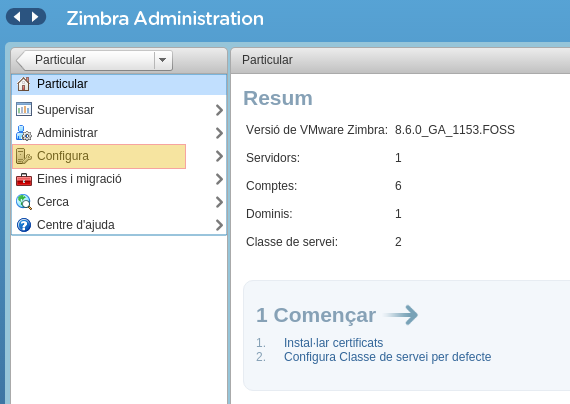
\includegraphics[clip,scale=0.5]{screenshots_admin_ca/Step1-1}
\par\end{centering}

\caption{\label{fig:Pas 1}Finestra inicial de la consola d'administraci�,
pestanya \textbf{\emph{Configura}}}
\end{figure}


\item Seguidament anar a l'apartat \textbf{\emph{Zimlets }}(veure figura
\ref{fig:Pas 2}).


\begin{figure}[H]
\begin{centering}
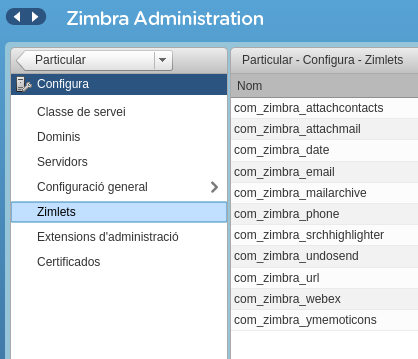
\includegraphics[clip,scale=0.5]{screenshots_admin_ca/Step1-2}
\par\end{centering}

\caption{\label{fig:Pas 2}Panell de configuraci�, apartat \textbf{\emph{Zimlets}}}
\end{figure}


\end{enumerate}
Un cop ens trobem al panell de configuraci� dels zimlets, hem de clicar
amb el bot� dret del ratol� sobre \textbf{\emph{com\_btactic\_bsmtp}}.
Es desplegar� un men� del qual hem de clicar l'opci� \textbf{\emph{Estat
de commutaci�}} (veure figura \ref{fig:Activar i desactivar zimlet}).\\
\\
Aquest procediment provocar� que l'estat del zimlet canvii d'activat
a desactivat o a l'inrev�s. Podem saber en quin estat es troba el
zimlet fixant-nos en la columna estat.\\
\\
Cal destacar que per tal que el zimlet estigui disponible l'estat
ha de ser \textbf{\emph{Activat}}, en cas contrari (estat \textbf{\emph{Desactivat}})
no estar� disponible.

\begin{figure}[H]
\begin{centering}
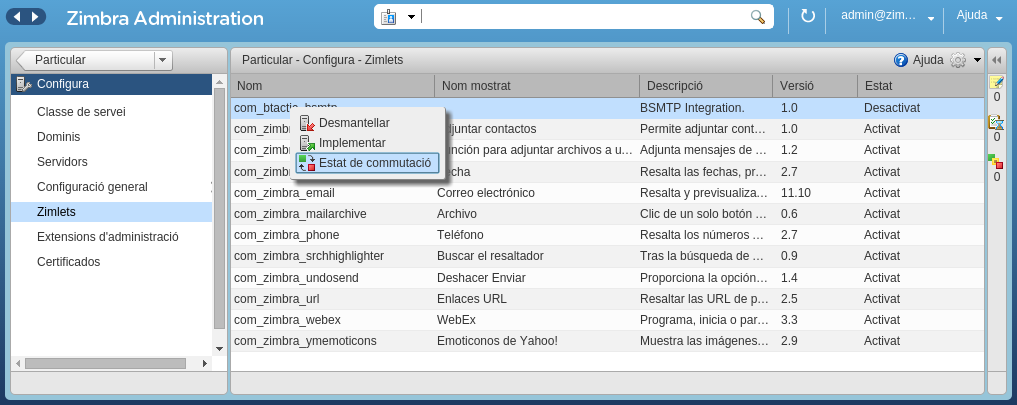
\includegraphics[clip,scale=0.5]{screenshots_admin_ca/Step3-1}
\par\end{centering}

\caption{\label{fig:Activar i desactivar zimlet}Activar/desactivar un zimlet}
\end{figure}



\section{Habilitar el zimlet a la classe de servei de l'usuari}

Per tal d'habilitar el zimlet a la classe de servei de l'usuari hem
d'entrar a la consola d'administraci�, pestanya \textbf{\emph{Configura
}}(m�s detalls al pas 1 de l'apartat \ref{sec:3 Activar i desactivar el Zimlet})
i un cop ens trobem al panell de configuraci�, hem de seguir els seg�ents
passos:
\begin{enumerate}
\item Clicar \textbf{\emph{Classe de servei}} al men� de l'esquerra i seleccionar
la classe de servei a la qual volem habilitar el zimlet (veure figura
\ref{fig:Configuraci=0000F3 classe de servei}).


\begin{figure}[H]
\begin{centering}
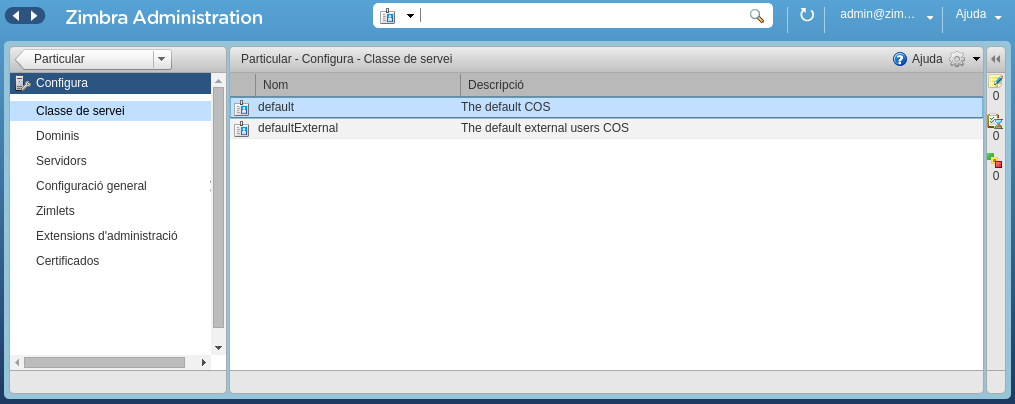
\includegraphics[clip,scale=0.5]{screenshots_admin_ca/Step4-1}
\par\end{centering}

\caption{\label{fig:Configuraci=0000F3 classe de servei}Configuraci� classe
de servei}
\end{figure}


\item Un cop hem seleccionat la classe de servei que volem editar, hem de
clicar la icona 
\includegraphics[scale=0.65]{screenshots_admin_ca/icon_config}
de la part superior dreta de la pantalla i sel�leccionar la opci�
\textbf{\emph{Edita}}\emph{ }(veure figura \ref{fig:Editar classe de servei})\emph{.}


\begin{figure}[H]
\begin{centering}
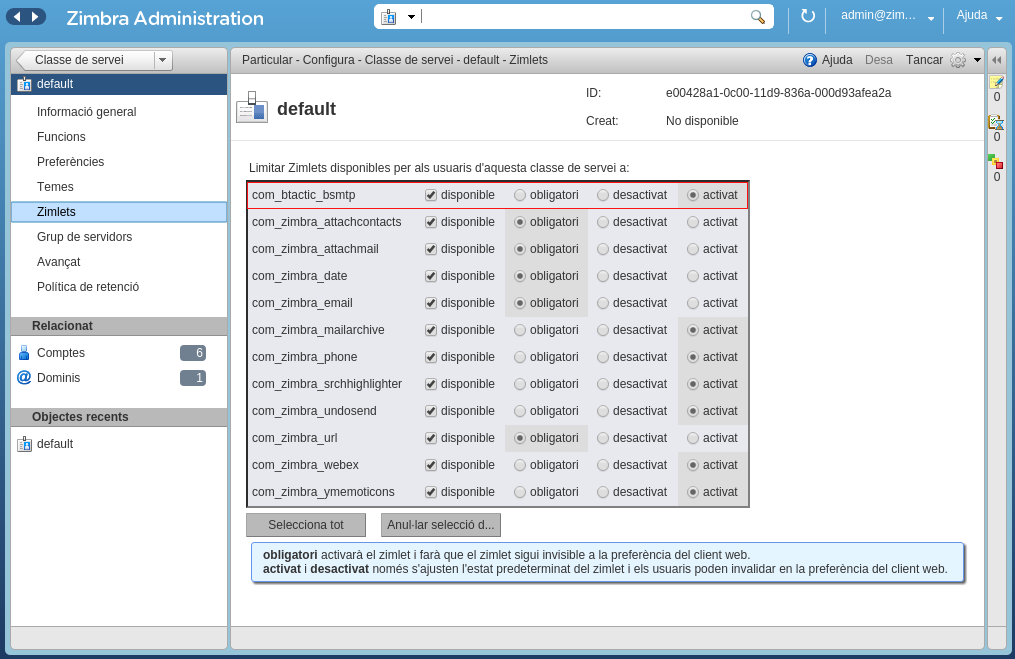
\includegraphics[clip,scale=0.5]{screenshots_admin_ca/Step4-2}
\par\end{centering}

\caption{\label{fig:Editar classe de servei}Editar classe de servei}
\end{figure}


\item Quan ens trobem a la configuraci� de la classe de servei que volem
editar hem d'anar a la secci� \textbf{\emph{Zimlets}} del panell de
l'esquerra i un cop all� editar la configuraci� de \textbf{\emph{com\_btactic\_bsmtp
}}seguint aquests crit�ris:

\begin{itemize}
\item \textbf{obligatori }activar� el zimlet i far� que el zimlet sigui
invisible a la prefer�ncia del client web. Per tant, l'usuari no podr�
deshabilitar el zimlet.
\item \textbf{activat} i \textbf{desactivat}\textbf{\emph{ }}nom�s defineixen
l'estat predeterminat del zimlet i els usuaris el poden habilitar
i deshabilitar.
\end{itemize}

Veure la figura \ref{fig:Configuraci=0000F3 dels Zimlets a la classe de servei}.


\begin{figure}[H]
\begin{centering}
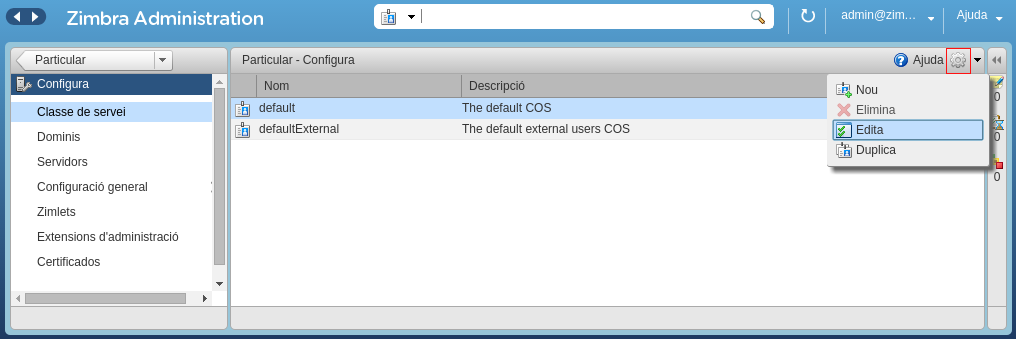
\includegraphics[clip,scale=0.5]{screenshots_admin_ca/Step4-3}
\par\end{centering}

\caption{\label{fig:Configuraci=0000F3 dels Zimlets a la classe de servei}Configuraci�
dels zimlets a la classe de servei}
\end{figure}


\end{enumerate}

\section{Codi font del zimlet}

El codi font i les distribucions del zimlet estan disponibles a \href{https://github.com/btactic/bsmtp}{https://github.com/btactic/bsmtp}
\end{document}
